\section{How a query-only monitor works}
\label{sec:monitor}

Each week the monitor asks: \emph{is there a group of accounts whose queries are jointly unusual, compared with how groups of ordinary users looked in past weeks?} Figure~\ref{fig:monitor} shows the pipeline; Appendix~\ref{sec:monitor-full} gives details.

\begin{figure}[t]
\centering
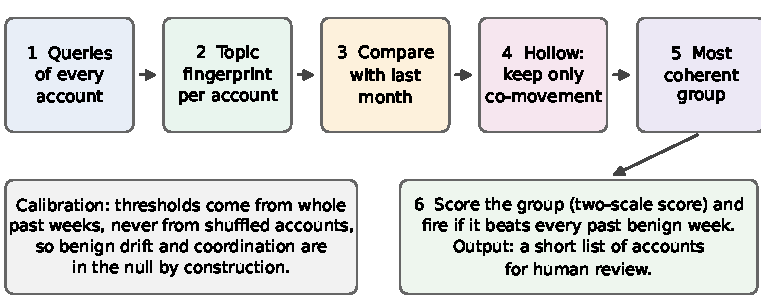
\includegraphics[width=\linewidth]{figs/monitor.pdf}
\caption{The monitor. Each account's queries become a topic fingerprint, compared with last month's traffic; hollowing keeps only how accounts co-vary; the most coherent group is scored against every past benign week.}
\label{fig:monitor}
\end{figure}

\paragraph{Fingerprints and whitening.} Each query is embedded (MiniLM; \citealp{wang2020minilm,reimers2019sbert}). An account's queries $x_1,\dots,x_{n_a}$ are summarised by random Fourier amplitudes $\rho_a(\omega_j)=\sum_i e^{-\mathrm{i}\,\omega_j\cdot\varphi(x_i)}$ \citep{rahimi2007random}: each random frequency probes one direction and scale of topic space, and an account that keeps returning to one region produces large, aligned amplitudes. Each account is then \emph{whitened} against the benign traffic of the four preceding weeks, $y_a=\Sigma^{-1/2}(\rho_a-n_a\mu)/\sqrt{n_a}$, so that an account sending ordinary queries has identity covariance however popular its topics are. The lagged reference absorbs slow drift.

\paragraph{Groups that move together.} Stacking the $y_a$ into a matrix $Y$ gives the cross-account matrix $C=YY^\top/r$. Independent accounts produce a random-matrix spectrum \citep{marchenko1967distribution}; a campaign whose accounts jointly concentrate adds a spike whose eigenvector points at the colluders \citep{baik2005phase}. The detector takes the fewest accounts carrying half of the top eigenvector's weight as its candidate group $G$ and scores it with the \emph{two-scale score} $T_{\rm 2s}(G)=\log\Sb_{h=4}(G)-\log\Sb_{h=0.5}(G)$, where $\Sb_h$ is the group's concentration at a coarse or fine bandwidth relative to independent queries. A group concentrated on a topic without the near-duplicate clumping of benign groups scores high. Because the score is a ratio within one group, weekly drift and population size largely cancel.

\paragraph{Hollowing.} $C$ has a weakness that turned out to matter: its diagonal holds each account's own concentration, so an individually topical benign user can dominate the top eigenvector, and padding a colluder with natural text shrinks its contribution. The \emph{centred, hollowed} matrix
\[
R_c=\Delta^{-1/2}\bigl(\tilde Y\tilde Y^\top-\Delta\bigr)\Delta^{-1/2},\qquad \Delta=\mathrm{diag}\bigl(\|\tilde y_a\|^2\bigr),
\]
where $\tilde Y$ is $Y$ with its mean row removed, deletes each account's self-term, normalises every account to unit length and removes the week's common drift \citep{cai2021subspace,zhang2022heteroskedastic}. Its top eigenvector picks accounts whose deviations \emph{point the same way}, however large or small. We call selection on $R_c$ followed by the two-scale score \emph{hollowed selection}. \emph{Multi-outlier selection} scores a group from every eigenvector of $R_c$ above the random-matrix bulk (up to 20) and keeps the largest score, $T_{\max}$.

\paragraph{Calibration.} We never build the null by shuffling accounts or queries, which destroys exactly the benign coordination the test must tolerate. Each threshold is the $(1-\alpha)$ quantile of the same statistic over \emph{whole} past weeks---the eight preceding weeks (\emph{rolling}) or all prior weeks (\emph{conformal})---each whitened against its own lagged reference. The spectral step costs $O(r^3)$ for $r$ whitened components, independent of the number of accounts; a weekly window took about 0.2\,s on one T4 GPU.

\paragraph{Baselines.} A whole-window shift test (the \emph{global stream}), the MMD \citep{gretton2012kernel} traffic-window test of \citet{liu2026embarrassingly}, per-account and Higher Criticism tests \citep{donoho2004hc}, Fraudar \citep{hooi2016fraudar}, a volume test, classifiers and topic statistics on the selected group, and a scan of topic-cell volumes, all with the same references and calibration.
